\chapter{Trace analysis}

In this chapter we describe how we process the execution traces to find execution differences
and, in turn, detect anti-adblockers.

\section{Parsing}
Although the format presented in Chapter \ref{v8-instrumentation} is really simple, parsing it can prove challenging.
The sole reason is the size of the files. It is really common for websites to produce files of size in the range of a few gigabytes.
Some can even output as much as 48 GB in about 2 minutes!

The analyzing program was written in Haskell \cite{haskell:main-page}.
Haskell is a purely functional, lazy, statically typed language.
It has been chosen because it is relatively easy to write parsers in a language like this.
Further, static typing with pattern matching proves convenient when manipulating well-structured data like log entries.
Last but not least, automatically derived instances
\footnote{Without going into details, type classes in Haskell are a bit like interfaces in 
object-oriented languages, e.g., the \texttt{Ord} class defines objects that can be ordered}
help avoid writing tedious code and focus on implementing non-trivial parts.

All that being said, Haskell is a bit like C\texttt{++} -- inexperienced user can easily make mistakes
that render the code slow and memory-greedy.

The logging format is described in Section \ref{v8-bytecode-injection}.
Each entry consist of an event type and several locations. Each location comprises
a function name, a source file and a position within the file.

At first, an internal format for the event was exactly the same. One object consisted of
two strings and two numbers (it could be one number, but this way line and column info
logging can be turned on any time).

The first mistake, specific to Haskell, was the use of the \texttt{String} type to represent the function and the file
names. The use of the default \texttt{String} to represent textual data makes the code inefficient 
because it is a linked lists of \texttt{Char}s, i.e. to store one character, 9 bytes of memory are used.
This representation is so inefficient that it is not even worth trying to profile it.

That error was fixed by changing the representation to the \texttt{ByteString} type from the \emph{bytesting} 
package \cite{haskell:bytestring}. \texttt{ByteString}s are represented internally as real byte arrays,
not linked lists. 
This change was accompanied by a rewrite of the parsing code to \emph{attoparsec} \cite{haskell:attoparsec}
which can operate on input \texttt{ByteString}s.

The code was much less memory-consuming and faster but it still seemed to consume too much memory.
Profiling proved that suspicions were warranted. The profiling diagram is shown on Figure \ref{fig:bytestring-lazy}. 
All the profiling diagrams in this section were collected by running the analyzing program on the same set of 6 input files.
The first three files occupy 48MB each, the last three -- 4MB each.
All the files combined occupy around 150MB of space, while the peak memory usage of the program 
was above 900MB of memory.

\begin{figure}[hbt!]
 \centering
 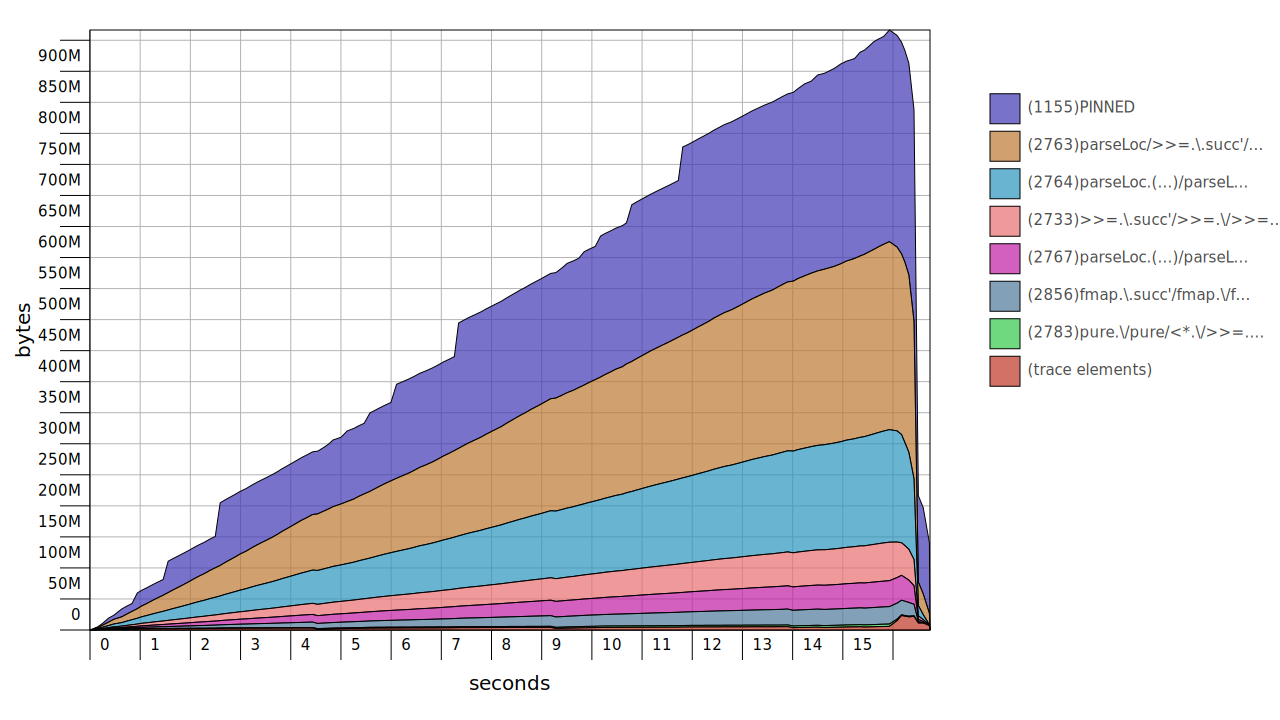
\includegraphics[width=\textwidth]{png/bytestring-lazy}
 \caption{Memory usage of the first implementation using the \texttt{ByteString} type as the internal strings representation}
 \label{fig:bytestring-lazy}
\end{figure}

Pinned memory seemed to be never freed during the execution. 
Also, traces seemed to reside in memory for too long and occupy too much space. 

The first problem was a reflection of how Haskell keeps \texttt{ByteString}s.
They are stored in pinned memory, which is kept on a heap but 
not managed by a garbage collector \cite{haskell:shortbytestring-and-text} and cannot be moved around.
As a result, it leads to fragmentation of the heap and it cannot be effectively managed.
The fix turned out to be simple. There is a more suitable storage format -- \texttt{ShortByteString} 
(also part of the \emph{bytestring} package). Objects of this type are managed
by the GC and stored just like usual heap objects, which can be moved around and easily garbage collected.

The second problem was harder to track down. This time the cause was the laziness.
Laziness can improve the performance when some objects are never used and the language never needs to fully compute them. 
However, when we know that all objects will eventually be used, it is more efficient
to calculate them as soon as possible. The enforcement of eager evaluation seems to be an obscure
feature, but it can significantly reduce memory consumption in certain situations.
The improvement was visible (cf. Figure \ref{fig:shortbytestring-strict}) but it was not the end, 
as the peak memory usage of almost 240MB was notably larger than the total trace files size.

\begin{figure}[hbt!]
 \centering
 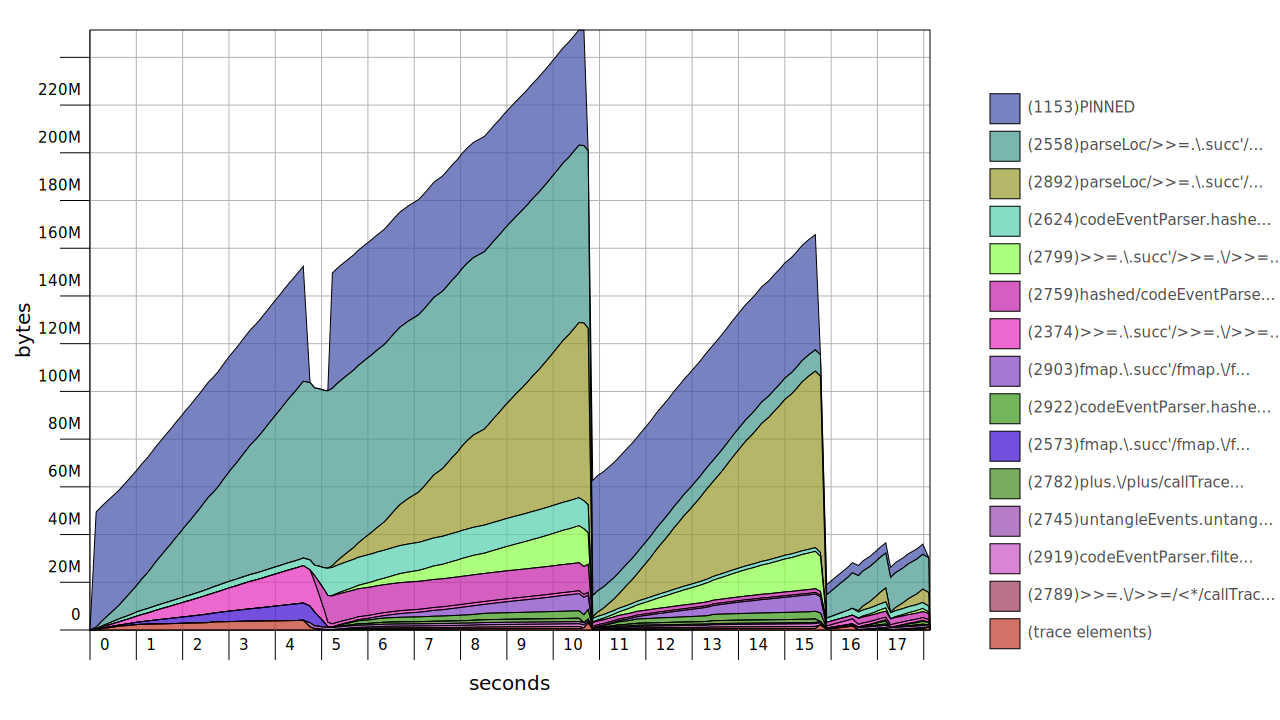
\includegraphics[width=\textwidth]{png/shortbytestring-strict}
 \caption{Memory usage after switching to the \texttt{ShortByteString} type and forcing the eager evaluation}
 \label{fig:shortbytestring-strict}
\end{figure}

It seemed suspicious that the entire file had to be kept in memory to be parsed 
(pinned memory on Figure \ref{fig:shortbytestring-strict} represents input files read into memory). 
After all, if the parser was written in C\texttt{++}, probably one line at a time would be read and processed. 
So why did the parser in Haskell consume so much memory?

This is what \emph{attoparsec} documentation states about the incremental input:

\begin{displayquote}
Note: incremental input does not imply that attoparsec will release portions of its internal state for 
garbage collection as it proceeds. Its internal representation is equivalent to a single ByteString: 
if you feed incremental input to a parser, it will require memory proportional to the amount of input you supply. 
(This is necessary to support arbitrary backtracking.)
\end{displayquote}

So, our parser kept the whole file contents in memory to be able to backtrack. But it was not necessary with
such a simple format. Fortunately, it was possible to alter this behaviour.
At that time, the parser tried to parse the entire file into a list of events. To make sure that it can backtrack,
it kept the whole input in memory. Instead, we asked the parser to parse only one event. 
It did it and returned a part of the input that was not parsed yet. We repeated that in a loop
and the parser never retained more than just a few kilobytes of memory. 
Figure \ref{fig:single-event} shows the improvement.

\begin{figure}[hbt!]
 \centering
 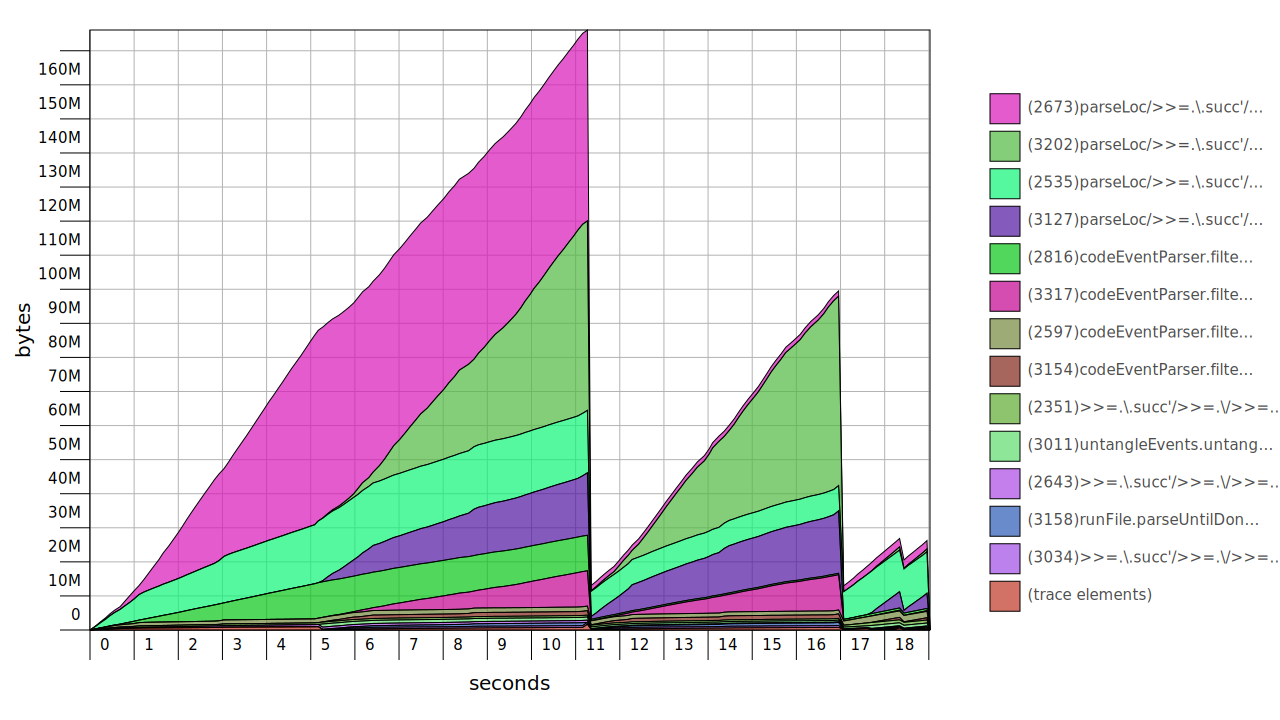
\includegraphics[width=\textwidth]{png/single-event}
 \caption{Memory usage after preventing the parser from keeping the entire input file in memory}
 \label{fig:single-event}
\end{figure}

Last but not least, the internal representation of the event could be greatly improved.
Locations consist of file names and function names. But both sets are limited!
Usually there are only a few sources containing just a few hundreds of unique functions. 
We can create a map of all source and function names and just keep the appropriate identifiers in location objects.
Just 4 numbers instead of 2 strings and 2 numbers!

This representation also has another major benefit -- comparisons of such objects are much faster.

The final memory consumption is presented on Figure \ref{fig:strings-map}.

\begin{figure}[hbt!]
 \centering
 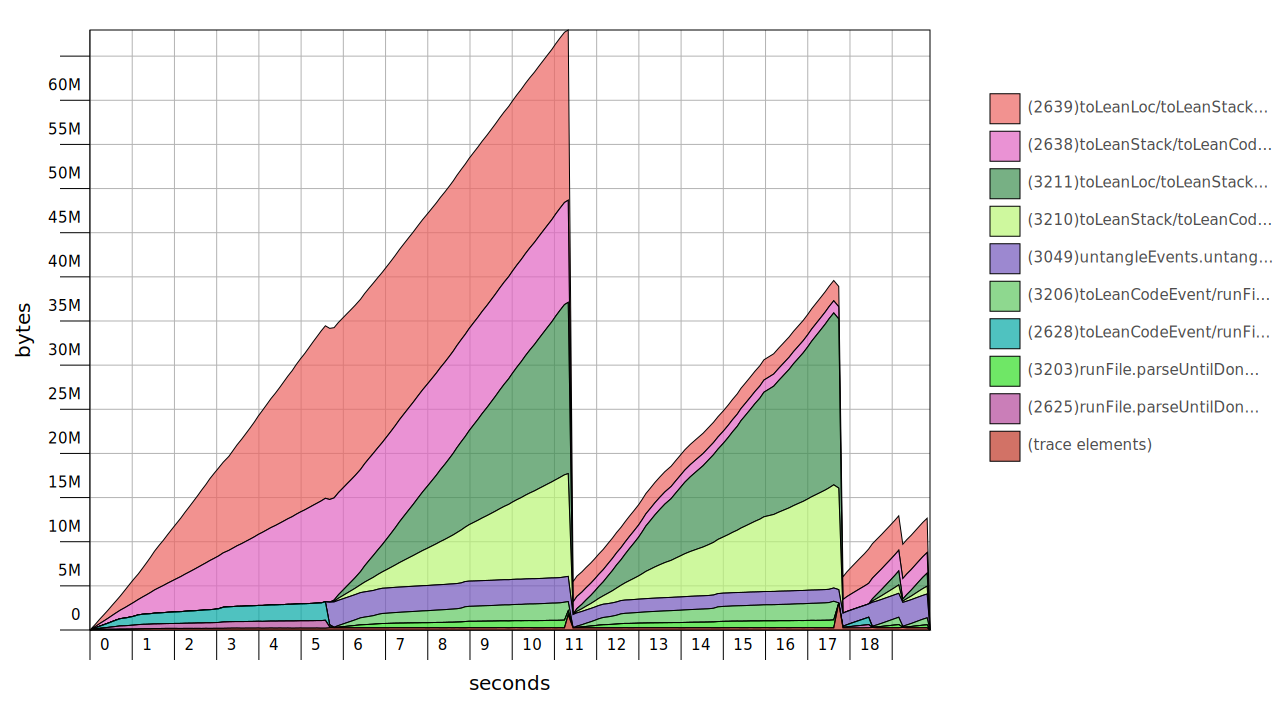
\includegraphics[width=\textwidth]{png/strings-map}
 \caption{Final memory usage of the analyzing program}
 \label{fig:strings-map}
\end{figure}


\section{Trace untangling}
Due to the nature of the JavaScript execution model (see Section \ref{js-exec-model}), execution events
corresponding to different JavaScript events or functions can be intertwined.

For this reason, all events forming a trace have to be untangled into subtraces, each corresponding
to one script or callback. 

Let us recall that all events are logged by our instrumented Chromium with their call stacks.
Now, we have three cases:
\begin{itemize}
  \item The event is a function entry with an empty call stack -- it starts a new subtrace.
  \item The event is a function exit removing the last item from the stack -- it ends a subtrace.
  \item Any other event -- it is a continuation of a subtrace whose last event has the same call stack.
\end{itemize}

Naturally, some care has to be taken to ensure that the right stack is compared. Some events change the
call stack, e.g., a function entry and exit, some do not, e.g. "if statement -- then".
Here, the stack from the moment just after the event occurred is saved and it is appropriately modified 
(the stack can grow or shrink by exactly one location or remain unchanged) when comparing
with the past events' stacks.

Listing \ref{alg:untangling} presents the pseudocode of the algorithm.

\lstinputlisting[language=Pseudocode, caption=Pseudocode of the trace untangling algorithm, label=alg:untangling, mathescape=true]{algorithms/untangling.alg}

The above code is rather uncomplicated, but it is slow when implemented naively.
The critical part is finding the trace with the right stack in \emph{findMatchingSubtrace}.
To make it fast, two things were done:
\begin{itemize}
  \item The location objects are just 4 numbers instead of 2 strings and 2 numbers. This makes stack comparisons
           one or two orders of magnitude faster.
  \item The open traces are kept in a map indexed by a stack of the last event. 
  			The lookup cost becomes logarithmic instead of linear. This optimization is especially important when there are lots
  			of intertwined subtraces. It should also be noted that this optimization alone
  			would not help much if stacks comparisons were slow.
\end{itemize} 

One last caveat -- it is possible to enter a function in JavaScript and never return from it.
When an exception is thrown and there is no catch block inside a function, the error will
be propagated higher and possibly multiple functions can be left without any of them returning any value.
The throw events are not logged, therefore this situation has to be taken care of
in the analyzing program. The solution is the following: when there is no open subtrace with a matching stack,
we check if some stack matches if we remove some elements from its top.
If so, then we assume that it is due to the try-catch block.


\section{Trace alignment}
\label{trace-alignment}

Trace alignment is a technique of identifying execution differences between two runs of the same program.
To be able to align two traces, events in both have to be assigned execution indices.
In our case the execution index is the event type, its location, and the stack at the time of its occurrence.
In this thesis the term "execution index" is often used interchangeably with the execution event as everything that is
logged when an event occurs is the index.

The algorithm used in this implementation is based on the work by Johnson et al. \cite{ieee:alignment-and-slicing}
The result of the trace alignment is an execution trace diff. It is a list of events of three kinds:
\begin{itemize}
  \item Common -- an event that occurred in both traces.
  \item Left -- an event that occurred only in the left-hand trace.
  \item Right -- an event that occurred only in the right-hand trace.
\end{itemize}

Each diff event includes the associated execution event.
Listing \ref{alg:alignment} present the pseudocode of the algorithm.

\lstinputlisting[language=Pseudocode, caption=Pseudocode of the trace alignment algorithm, 
                       label=alg:alignment, mathescape=true]{algorithms/alignment.alg}
                       
The algorithm output includes a score, which is a number of common events.
This concept is present in the original article and its purpose 
is explained in Section \ref{trace-matching}.

The algorithm is rather simple. We assume that matching traces have to start with the same
event. If they do not (lines 5-6), we just terminate and return a score of -1, 
which signifies that the traces do not match.

Apart from the case when one of the traces ends, there are only two cases:
\begin{itemize}
  \item Both unprocessed traces start with the same event (this implies that stacks are equal) -- line 20 -- in this case
  			we add an event of type Common and remove one event from both lists
  \item The top events do not match (lines 25 and 28) -- in that case the event with larger stack is processed first.
           The reasoning is the following. The bottom of the larger stack is the same as the shorter stack.
           If we first process the shorter stack and if it shrinks, we lose some common events.
           It we process the larger stack first, the shorter one is "frozen". The larger stack may grow, but it doesn't matter
           since it is already divergent. When it shrinks to the size of the shorter stack, it is a re-convergence point.
\end{itemize}


\section{Trace matching using the Stable Marriage Problem}
\label{trace-matching}

We already know how to align two traces (Section \ref{trace-alignment}), but we have not
answered a different question -- which pair of subtraces should we align?

This thesis presents a novel approach which uses the Stable Marriage Problem (SMP) to answer this question.
First, we define what the SMP is and later explain how it is adapted to our needs.

The original statement of the problem is the following: 
given equally sized sets of men and women and their matrimonial preferences,
find a stable matching, i.e. matching in which there exists no pair of a man and a woman 
in which they both would have better partner than the currently assigned one.
The problem can be solved using the Gale-Shapley algorithm \cite{gale-shapley}. 
Listing \ref{alg:gale-shapley} presents its pseudocode.

\lstinputlisting[language=Pseudocode, caption=Pseudocode of the Gale-Shapley (deferred acceptance) algorithm, 
                       label=alg:gale-shapley, mathescape=true]{algorithms/gale-shapley.alg}

This is how the SMP is used to solve the subtrace matching problem:
\begin{itemize}
  \item In the first phase all pairs of subtraces are aligned and similarity scores (a number of common events) 
  		    are calculated -- the score is the marital preference.
  \item In the second phase, an adapted Gale-Shapley algorithm is run and only the matched subtraces
           are used. Their diff is retrieved from a special map as it was calculated and stored there in the first phase.
\end{itemize}

All men have a list of women sorted by their preferences (from highest to lowest).
At the beginning everyone is free. Then, in each round each free man $m$ proposes to the first woman $w$ he has not yet proposed to.
The woman can reply "maybe" if she is free or is engaged to $m'$ and prefers $m$ over $m'$. Otherwise, she rejects.
So women only "trade up" and men propose whenever they are free to the best possible partner.
In the end everybody is engaged and the marriages are stable.

The time complexity of this algorithm is $O(n^2)$, where $n$ is the number of men or women.
There is at most $n$ rounds (some man proposes to every woman) and in each round
there are at most $n$ proposals made.

In the original problem statement the number of women is equal to the number of men
and everybody gets engaged in the end.
In our case the number of men and women does not have to the same. We assume that
the more numerous group has the role of women. 
We allow some pairs of men and women to not match each other (the preference score equal to $-1$),
therefore in the end some people may not be engaged.

Let us see what happens with these two adjustments and the same procedure as in the original version:
\begin{itemize}
  \item The men should still propose in the order from the highest preference to the lowest. 
  			All men will still get the best possible match this way, 
  			because all women that rejected must have had some better options.
  \item The women should accept anybody when they do not have any tentative match and
           trade up later. If there is a man that a woman prefers over the current match and he did not
           propose, he must have had someone who he preferred more and who accepted.
\end{itemize}

Consequently, the algorithm is almost the same. The only exception is that men do not propose to women with score -1.
Also, the result is different -- in the end there usually will be many people without a pair. 
However, those who are paired form stable marriages.

Such a usage of the Deferred Acceptance algorithm allows us to form the best pairs of subtraces to align.
There is no point in aligning the traces that do not have the same initial event (the aligning algorithm has to
start from an anchor point), so we skip the pairs with the assigned score equal to $-1$. Further, the best pairs are
selected by the number of common events. If two traces A and B are exactly the same, the only possibility that they will
not be matched is when there is some longer trace C that contains the entire A and B. But, if there is also a longer trace D
that contains the entire A and B, it is very likely that the extra part will be matched with an extra part of C and,
in consequence, C and D will be matched. If there is no such a trace D and C is matched with either A or B, it is still
fine as we have more calls to some function in one group and we cannot be sure which subtraces truly
correspond to each other.


\section{Artificial examples}

This section presents how the above algorithm works on a few simple, hand-crafted examples run in a standalone V8.

The first example is based on our already-familiar example of the \emph{factorial} function (Listing \ref{js-factorial}).

First, we call the function with $n=3$, then with $n=4$ and compare the traces.
This demonstrates how "if-then-else" divergences are detected.
Listing \ref{diff:factorial} shows the output of the program.

We see that after 3 \emph{factorial} calls the traces diverge and one of them takes the "else"
branch and makes one more recursive call (lines 19-30). The other takes the "then" branch (lines 31-33).
After that one extra recursive call both traces immediately reconverge (line 34).

\lstinputlisting[language=TraceDiff, caption={A trace diff of the \emph{factorial} function run with $n=3$ and $n=4$},  label=diff:factorial]{out/factorial.diff}

The next example demonstrates that sometimes it is possible to find a divergence even when
the built-in functions are involved. Listing \ref{js:map} is a short example involving \emph{Array.prototype.map}.
In the first run the built-in function is called with an array of length 3, in the second -- the array contains one item less.
Listing \ref{diff:map} shows the diff. We can see that in one run \emph{multiplyByTwo} is entered 2 times and in the
other -- 3 times. Naturally, if the arrays were of the same length, but with different content, this difference would not
be caught this way.

\lstinputlisting[language=JavaScript, caption=A simple JavaScript example of the \emph{Array.prototype.map} usage, label=js:map]{js/map.js}

\lstinputlisting[language=TraceDiff, caption={A trace diff of the \emph{Array.prototype.map} run with arrays of length 3 and 2},  
						label=diff:map]{out/map.diff}
						
The last example demonstrates the generator-related events in action.
Listing \ref{js:generators} shows an example of \emph{factorial} rewritten to use generators. It is run two times, with $n=2$ and $n=3$.
Listing \ref{diff:generators} shows the resulting diff. We can see that when the generator is created, the \texttt{FunctionEnter} event
is emitted, followed by the \texttt{GeneratorSuspend} (lines 7-12). Events \texttt{GeneratorEnter} and \texttt{GeneratorYield} are used 
only when the \emph{Generator.prototype.next} is called. Last but not least, the \texttt{GeneratorYield} event is always followed by 
\texttt{GeneratorSuspend}.

\lstinputlisting[language=JavaScript, caption=An example of JavaScript code using generators, label=js:generators]{js/generators.js}

\lstinputlisting[language=TraceDiff, caption={A trace diff of the generator-using \emph{factorial} function run with $n=2$ and $n=3$},  
						label=diff:generators]{out/generators.diff}

\section{Noise filtering}

One of the biggest challenges in the entire method is filtering the noise.
The noise on the website may come in many different flavours:
\begin{itemize}
  \item Some content can be based on Random Number Generators.
  \item The content may be dynamic and different with each refresh of the page, e.g., Facebook feed.
  \item Code that is not related to the website, e.g., trackers, analytics.
\end{itemize}

The difficult part is to filter out as much data as possible, without removing valuable information.

In the original paper authors collect redundant traces, diff together all positive traces (as defined in Section \ref{definitions}),
then also all negative traces, and generate a blacklist of execution divergences that are guaranteed to be noise.

In this thesis, we chose a different approach. The positive traces are all put together and the common subtraces are extracted.
The same thing is done with the negative traces. 
At the end, the whole SMP and alignment analysis (see Sections \ref{trace-alignment} and \ref{trace-matching}) 
is run only on these common subtraces.

The effectiveness and limitations of this approach are discussed in Chapter \ref{evaluation}.
